\documentclass[11pt,a4]{article}
\usepackage[a4paper,includeheadfoot,margin=2.54cm]{geometry}
\usepackage{graphicx}
\usepackage{rotating}

\author{Stuart Reilly - 2258028}
\title{Safety Critical Systems Assessed Exercise (H)}
\date{\today}

\begin{document}
\pagenumbering{roman}
\maketitle
\tableofcontents
\pagenumbering{arabic}

\pagebreak
\section{Risk Assessment Tool}
Figure \ref{fig:tool} shows a visual representation of the tool.
The risk assessment tool is based on the technique of fault trees.
By setting the probabilities of the base events to the values shown in Figure
\ref{fig:values}, the probability of train derailment is roughly $0.3$.
The probabilities used are for the modern probability, historic probabilities are
lower, and as such, the probability of train derailment is lower.

\begin{figure}[h]
	\label{fig:values}
	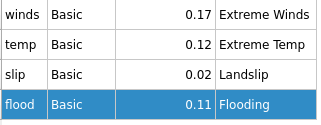
\includegraphics{probs}
	\caption{The modern probabilites of the base events}
\end{figure}

\begin{figure}[h]
	\label{fig:tool}
	\vspace{-2cm}
	\begin{sideways}
		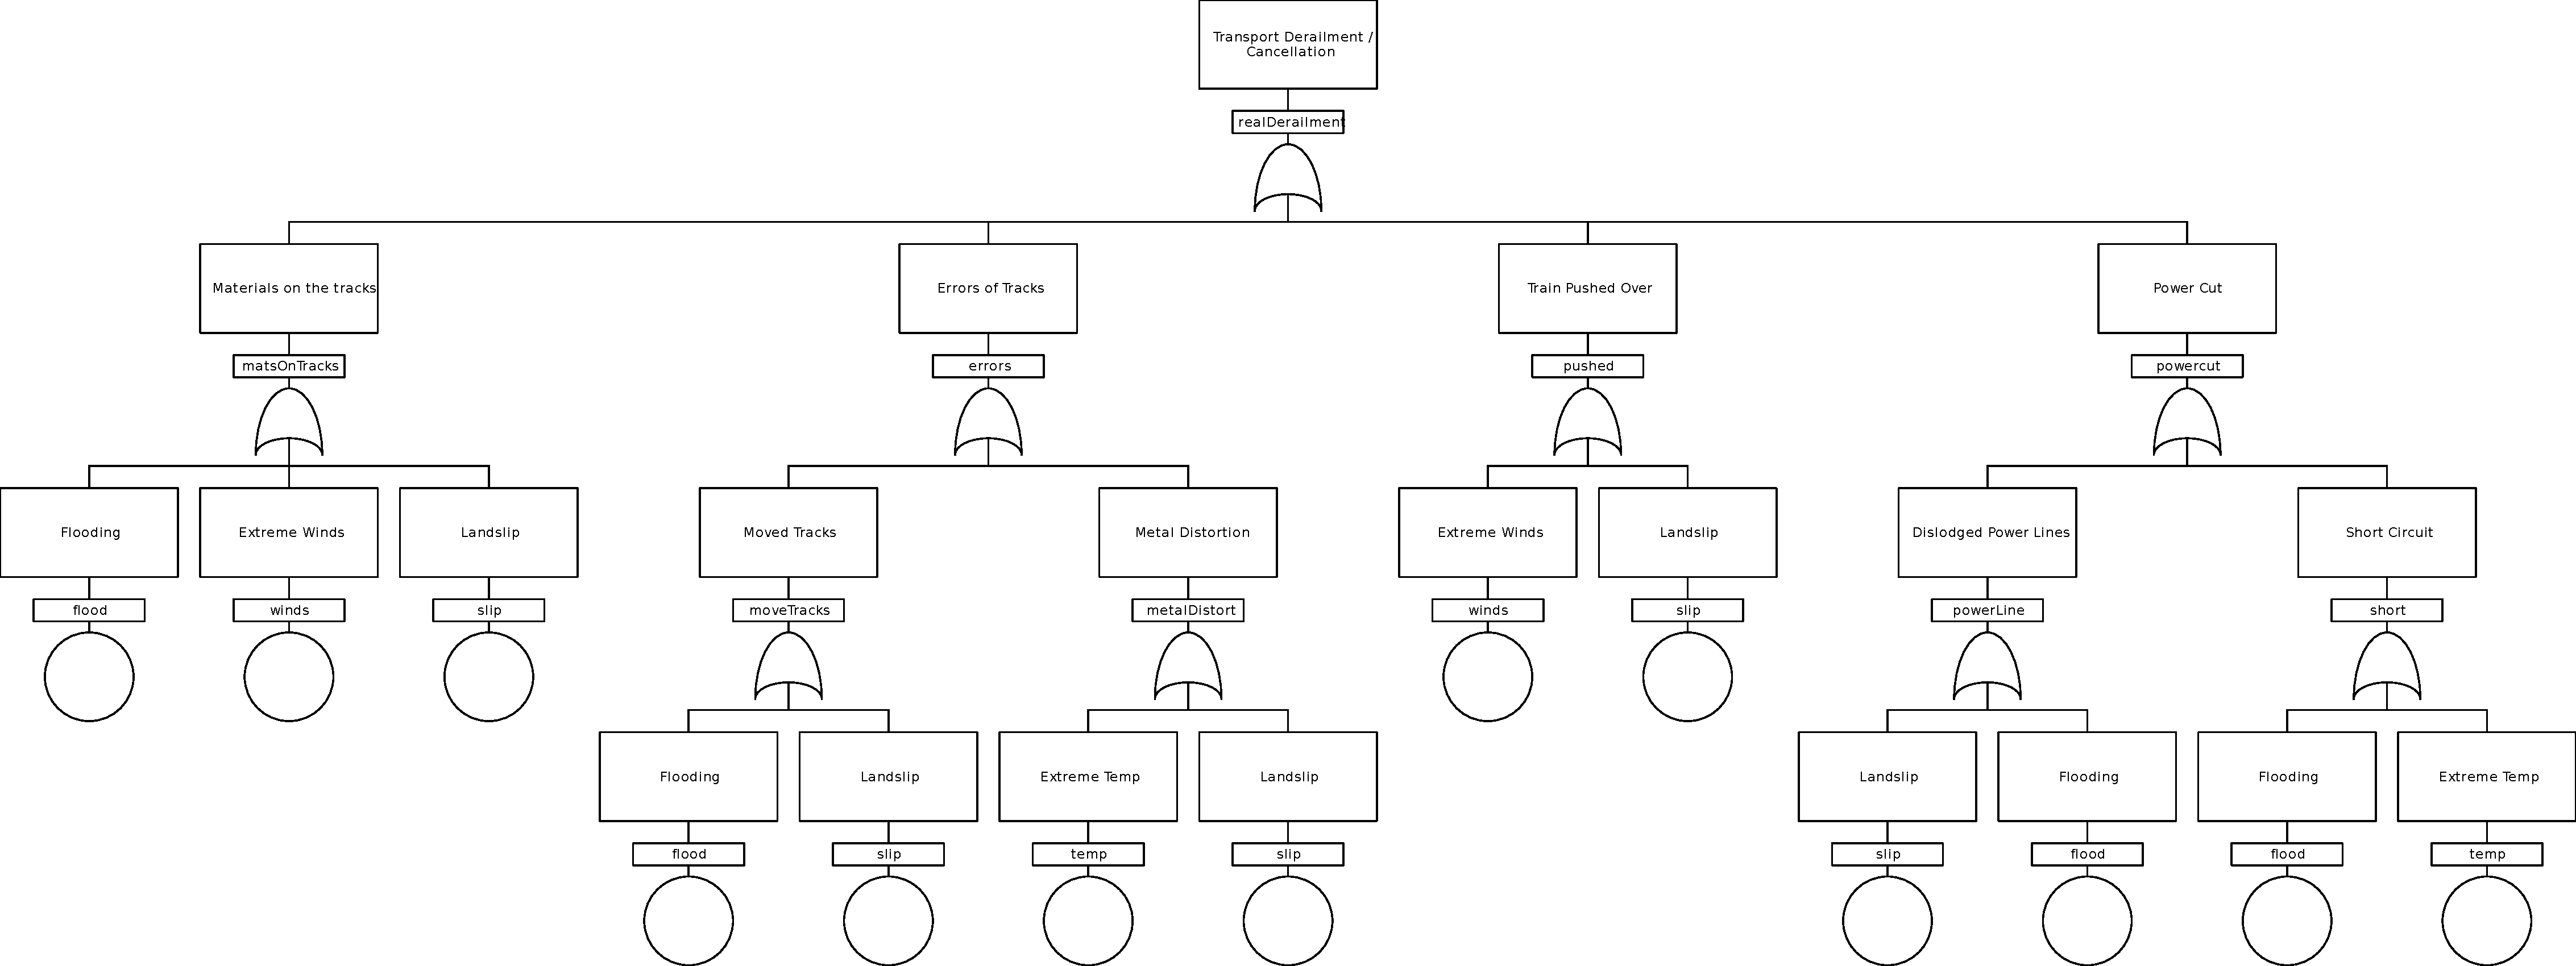
\includegraphics[width=25cm]{faulttree}
	\end{sideways}
	\caption{The tool}
\end{figure}

\section{Evaluation of Tool}
This tool may not even fulfil the specification for the coursework, but since
the coursework had a information-sparse specification, it could well be correct.
As for the usability, it was not taken into account for the tool.
It is intended to be as obtuse as possible.
As such, it is not an interactive tool, more of an example of a possible technique
middle management cunts could use.

\section{Results}

\section{Conclusion}
This coursework was far too open ended and extensive for the equivalent
of 2 credits, especially during the final year of a degree with an already
extensive dissertation.
The topics discussed in the lectures are extremely interesting and important,
but this coursework has single-handedly destroyed any semblance of enjoyment
for this course overall.

\end{document}
